% ${framed}

\documentclass[9pt,addpoints]{exam}
\usepackage{dsfont}
\usepackage{amsfonts}
\usepackage{amsmath}
\usepackage{array}
\usepackage{tabularx}
\usepackage{etoolbox}
\usepackage{eso-pic}
\usepackage{hyperref}
\usepackage{color}

\usepackage[letterpaper,top=1.55cm, bottom=3.5cm, outer=4cm, inner=3cm,
            heightrounded, marginparwidth=0cm,marginparsep=1cm]{geometry}

\newtoggle{compress}
\toggletrue{compress}
%\togglefalse{compress}

\hypersetup{
  pdftitle={Test 3 for Math 1113, Fall 2018},
  pdfsubject={Precalculus},
  pdfauthor={PBergonio},
  anchorcolor = {red},
  colorlinks = {true},
  %% pdfpagemode={FullScreen}
}
 

\usepackage{tikz}
\usepackage{pgf}
\usepackage{pgfplots}
\usepgfplotslibrary{fillbetween}
%%\pgfplotsset{width=7cm}
\usepgfplotslibrary{patchplots}


%%\oddsidemargin=-0.5in
%%\evensidemargin=-0.5in
%%\textwidth=7.5in

%%\topmargin=-0.75in
%%\textheight=9.5in

\pagestyle{plain}
 \reversemarginpar

\pointpoints{pt}{pts}
\bracketedpoints

\def\Course{Math 1113}
\def\NumSec{}
%% \def\time{12:00pm-12:50pm}
\def\Date{Fall 2018}
\def\test{Test 3 - Version A}
\def\version{B}


 \pagestyle{headandfoot}
 \headrule
 \firstpageheader{\bf 
   University of Georgia \\ % 
   Department of Mathematics}
 {\bf\Course \\ \test  }
 {\Date}
  \runningheadrule
  \runningheader{\Course}
               {\test %%, Section \NumSec
               }
               {\Date}
 \footrule
 \firstpagefooter{\version}
                 {Page \thepage\ of \numpages}
                 {}
 \runningfooter  {\version}
                 {Page \thepage\ of \numpages}
                 {\rule{0cm}{.35cm} Points earned: \hbox to
                 1cm{\hrulefill} \\  %
                  out of a possible \pointsonpage{\thepage} points}
%%%%%%%%%%%%%%%%%%%%%%%%%%%%%%%%%%%%%%%%%%%%%%%%%%%%%%%%%%%%%%%%%%%
 \extrawidth     { 1.00in}
  \extraheadheight{0.15in}%[-0.30in]{-0.30in}
 \extrafootheight{-0.41in}
 \addpoints
 %%%%%%%%%%%%%%%%%%%%%%%%%%%%%%%%%%%%%%%%%%%%%%%%%%%%%%%%%%%%%%%%%%%

\newcommand{\pointBox}{\marginpar[\begin{minipage}{1cm}\hfill\vspace*{1cm}
    ~ \\ \rule{1.5cm}{0.2mm}\end{minipage}]{~}}


\newcommand{\laplace}[1]{\makebox{$ {\cal L} \{ #1 \}$}}
\newcommand{\vi}{\makebox{$\vec{\imath}$}}
\newcommand{\vj}{\makebox{$\vec{\jmath}$}}
\newcommand{\vk}{\makebox{$\vec{k}$}}
\newcommand{\lp}{\left(}
\newcommand{\rp}{\right)}
%%\newcommand{\half}{\frac{1}{2}}




\begin{document}


%% <%include file="coverPage.template"/>

\noindent
\begin{tabular}{ll@{\hspace{3em}}ll@{\hspace{3em}}ll}
  %%%%\multicolumn{4}{l}{\textit{You must acknowledge that this is your
  %%%%work by signing:} } \\ %

  \multicolumn{4}{m{\textwidth}}{
  By providing my signature below  I acknowledge
  that I  abide by the University's academic honesty policy.
  This is my work, and I did not get any help from anyone else
  during the exam:} \\ [25pt] \\
  
  Name (sign):    & \rule{5cm}{0.2mm} & 
                                        Name (print):   & \rule{5cm}{0.2mm}  \\ [20pt]
  Student Number: & \rule{5cm}{0.2mm} \\ [20pt]
  Instructor's Name: & \rule{5cm}{0.2mm} & Class Time: & \rule{4cm}{0.2mm}
\end{tabular}


%%\bonustotalformat{Common Knowledge}

\vqword{
  \begin{minipage}[h]{5em}
    ~ \\Problem \\ Number \\ [-8pt]
  \end{minipage}
}
\vpword{
  \begin{minipage}[h]{5em}
    ~ \\ Points \\ Possible \\ [-8pt]
  \end{minipage}
}
%%\cvbpword{
%%  \begin{minipage}[h]{5em}
%%    ~ \\ Bonus \\ Points \\ [-8pt]
%%  \end{minipage}
%%}
\vsword{  \begin{minipage}[h]{5em}
    ~ \\ Points \\ Made \\ [-8pt]
  \end{minipage}
}
\vspace{0.8in}
\[
  \cos(\alpha + \beta) = \cos(\alpha) \cdot \cos(\beta) - \sin(\alpha) \cdot \sin(\beta)
\]
\vspace{1em}
\[
  \sin(\alpha + \beta) = \sin(\alpha) \cdot \cos(\beta) + \cos(\alpha) \cdot \sin(\beta)
\]


\newenvironment{nagging}%
  {\begin{itemize}%
    \setlength{\itemsep}{6pt}%
    \setlength{\parskip}{0pt}}%
  {\end{itemize}}

\vfill

\begin{tabular}{p{8cm}m{8cm}}
  \gradetable[v][questions]
  %%\partialgradetable{main}[v][questions]
  %%\partialbonusgradetable{bonus}
  %%\combinedgradetable[v][questions]
  &
    \begin{nagging}
    \item If you need extra space use the last page.

    \item Please show your work. \textbf{An unjustified answer may receive
        little or no credit.}

    \item If you make use of a theorem to justify a conclusion then
      state the theorem used by name.

    \item Your work must be {\bf neat}. If I can't read it (or can't
      find it), I can't grade it.

    \item The total number of possible points that is assigned for
      each problem is shown here.  The number of points for each
      subproblem is shown within the exam.

    \item Please turn off your mobile phone.

    %\item You are only allowed to use a TI-30 calculator. No other
    %  calculators are permitted.

    \item A calculator is not necessary, but numerical answers should
      be given in a form that can be directly entered into a
      calculator.
    \end{nagging}
\end{tabular}

\vfill



\bonuspointpoints{Point Common Knowledge}{Bonus}


\clearpage 

%% <%include file="defaults.template"/>
%% <%include file="overallreport.template"/>

\bonuspointpoints{Point Common Knowledge}{Points Bonus}

\clearpage


\begin{questions}

   \question A sector has radius $r = 23$ inches and interior angle $\theta = 2.4$ radians.  Answer the following.  Give an exact answer, or an answer correct to four decimal places.
   
    \begin{parts}
    \part[6]  Determine the perimeter of the sector.
\vskip 2in
    
    \part[6]  Determine the area of the sector.

\vskip 2in

  \end{parts}
  
     \question Give an exact value for the following expressions, or explain why the value does not exist.  Decimal answers without sufficient work will receive no credit.
   
    \begin{parts}
    \part[6]  $\cos(\arccos(2 \pi))$
\vskip 2in

    \part[6]  $\arcsin\left(\sin\left(\dfrac{13\pi}{8}\right)\right)$
\vskip 2in
  \end{parts}
      \iftoggle{compress}{\clearpage}
  
     \question[12] Determine the Domain and Range of the given functions.  Give your answer in interval notation.  You do not have to show your work.
     
\begin{center}     \begin{tabular}{| c | c | c | } \hline  & &  \\
     FUNCTION & DOMAIN & RANGE \\ & & \\ \hline & & \\
     
     \textcolor{white}{XXX}$f(x) = 4 - \sin^2(x)$      \textcolor{white}{XXX}& \textcolor{white}{XXXXXXXXXXXXXXXXX}& \textcolor{white}{XXXXXXXXXXXXXXXXXXX} \\ & & \\ \hline & & \\
     
     $g(x) = \arcsin(x)$ & \null & \null \\ & & \\ \hline & & \\
          
     $h(x) = \arctan(x)$ & \textcolor{white}{XXXXXXXXXX}& \textcolor{white}{XXXXXXXXXX} \\ & & \\ \hline
               
     \end{tabular}\end{center}
  


      
      
    \question[8]  Give an exact value for the following expressions.  Decimal answers without sufficient work will receive no credit.
    
    \[\cos(\arcsin(0.6) + \arccos(0.7))\]


  \iftoggle{compress}{\clearpage}

   \question Suppose that $3\pi/2 \leq \theta \leq 2\pi$ and $\cot(\theta) = -\dfrac{9}{13}$.  Answer the following:
   
    \begin{parts}
    \part[4]  Determine the \textbf{exact value} for $\cos(\theta)$.
\vskip 2in
    
    \part[4]  Determine the \textbf{exact value} for $\sin(\theta)$.
    
\vskip 2in


\part[8] Determine the value for $\theta$ that satisfies the given equation.  Give an exact answer, or an answer correct to four decimal places.

\end{parts}
  \iftoggle{compress}{\clearpage}


  
\question[15] The graph of a periodic function $f(x)$ is given below.  Determine a possible function for $f(x)$.  Make sure to show all your work.

\[\fbox{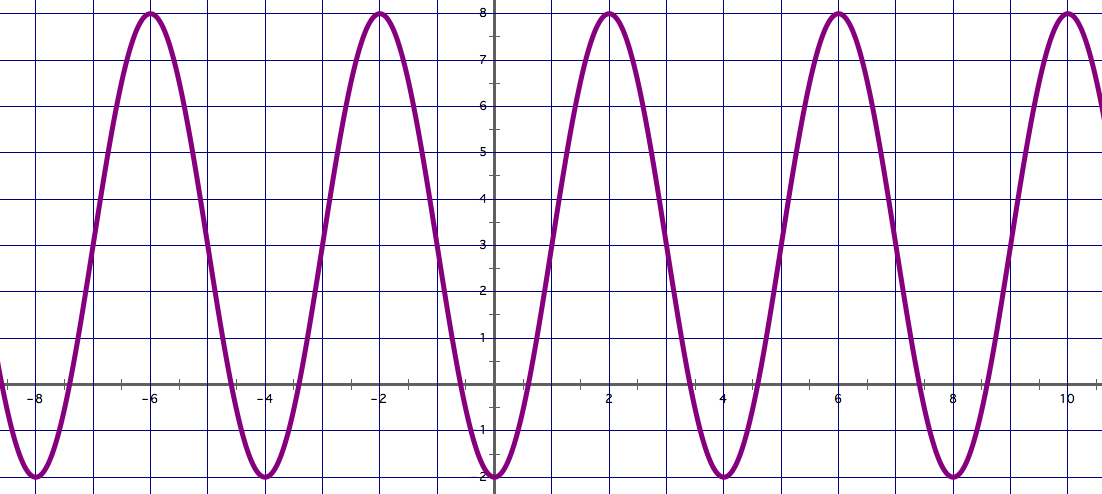
\includegraphics[width=6in]{T3F18.png}}\]


  \iftoggle{compress}{\clearpage}


\question[10] Use properties of trigonometry to show that the following equation is an identity.  

\[\displaystyle \frac{\cos^2(x) + 8}{\sin(x)} + \sin(x) = 9\csc(x)\]

  
  \iftoggle{compress}{\clearpage}
    

  \question[15] On my vacation to Los Angeles I took a helicopter tour and saw the iconic Hollywood Sign (45 ft tall) from a straight-line distance of 1500 ft. The angle of depression between me and the bottom of the Hollywood sign is $13.7^\circ$. What is my elevation, measured from the top of the Hollywood sign? 
  \begin{center}
    
\includegraphics[scale=4]{hollywood.jpg}
  \end{center}

  \iftoggle{compress}{\clearpage}

\end{questions}



Extra space for work. \textbf{Do not detach this page.} If you want us to consider the work on this
    page you should print your name, instructor and class meeting time below. \\ [10pt]
    Name (print): \rule{3cm}{0.2mm} Instructor (print):
    \rule{3cm}{0.2mm}  Time: \rule{3cm}{0.2mm}


    \iftoggle{compress}{\vfill}{~\\}



\end{document}


